%% Beamer-ported version of mru.tex ==
%% 
%% Original created 05-10-2008; ported to Beamer July 2025
\documentclass{beamer}

\pdfminorversion=7  % Allow higher PDF versions to fix inclusion warning

\usepackage{xcolor}
\usetheme{Copenhagen}  % Change to Madrid, Copenhagen, etc., for fancier look
% Define custom colors
\definecolor{electricblue}{RGB}{0,191,255} % Electric blue
\definecolor{creamyblue}{RGB}{173,216,230} % Creamy blue
\newcommand{\red}[1]{\textcolor{red}{#1}}
%\setbeamercolor{structure}{fg=electricblue} % Apply electric blue
\setbeamercolor{structure}{fg=creamyblue} % Uncomment for creamy blue

\usepackage[latin1]{inputenc}
\usepackage{amsmath}
\usepackage{cancel}
\usepackage{tikz}
\usepackage{graphicx}  % For images
\usepackage{lmodern}  % Fix font substitution warnings

\hypersetup{
pdfpagemode={FullScreen},
pdftitle={MRU e1: ver1},
pdfauthor={mmatex},
pdfcreator={mmatex},
pdfproducer={mmatex},
pdfkeywords={Movimiento,Rectilineo,Uniforme}}

%% You can insert definicions here..

%% DEFINICIONES MIAS..
%\def\psPiFour{12.566371}
%\def\psPiTwo{6.283185}
\def\psPi{3.14159265}
%\def\psPiH{1.570796327}
%\newdimen\pstRadUnit
%\newdimen\pstRadUnitInv
%\pstRadUnit=1.047198cm % this is pi/3
%\pstRadUnitInv=0.95493cm % this is 3/pi

%% Libreria de formulas %%%%%%%%%%%%%%%%%%%%%%%%%%%%%%%%%%%%
\input{lib/FORMULAS}
%% Libreria de Notas    %%%%%%%%%%%%%%%%%%%%%%%%%%%%%%%%%%%%
\input{lib/NOTASUNIDADES}

%________________________________________________________________(ult. col, 65)
% ==================== Titulo, autor, etc  ====================== 
\title{MRU e12: ver1}
\subtitle{MMaTeX - eScience}
\author{mmatex.com}
%________________________________________________________________(ult. col, 65)
%________________________________________________________________(ult. col, 65)

%%%%%%% Para pegar el log.. %%%%%%%%%%%%%%%%%%%%%%%%%%%%%%%
\logo{%
    \begin{tikzpicture}
        \node[opacity=0.2] {
\includegraphics[width=1cm]{images/citlogogrey.eps}};
    \end{tikzpicture}
}

%%%%%%%%%%%%%%%%%%%%%%%%%%%%%%%%%%%
%%% Comienzo del documento.. %%%%%%
%%%%%%%%%%%%%%%%%%%%%%%%%%%%%%%%%%%
\begin{document}
\maketitle
%%%%%%%%%%%%%%%%%%%%%%%%%%%%%%%%%%



%________________________________________________________________(ult. col, 65)
% ========================== slide1 ============================= 
\begin{frame}
\frametitle{Movimiento Rectil\'ineo Uniforme}
% 
% -Paragraph1 
%----------------------------------------------------------------
%----------------------------------------------------------------
% -Idea1 
% ============================================================== 
 La f\'ormula principal:

                                                               
% ============================================================== 
% -Idea2 
% ============================================================== 
 
{\huge \vmru}
\vNUa
                                                               
% ============================================================== 
% -Idea3 
% ============================================================== 
                                                               
                                                               
                                                               
% ============================================================== 
%----------------------------------------------------------------
%----------------------------------------------------------------
\end{frame}

%________________________________________________________________(ult. col, 65)
% ========================== slide2 ============================= 
\begin{frame}
\frametitle{MRU}
% 
% -Paragraph1 
%----------------------------------------------------------------
%----------------------------------------------------------------
% -Idea1 
% ============================================================== 

Recu\'erdalo por sus unidades:

% ============================================================== 
% -Idea2 
% ============================================================== 

\begin{equation*}
10\frac{\text{km}}{\text{h}} =
\frac{\text{Se recorren 10 km ({\red distancia})}}
{\text{en 1 hora ({\red tiempo})}}
\end{equation*}
                                                               
% ============================================================== 
% -Idea3 
% ============================================================== 
 
Las otras dos f\'ormulas que se derivan de (\ref{vmru}) son:

{\large \xmru \\ \tmru}
                                                              
% ============================================================== 
%----------------------------------------------------------------
%----------------------------------------------------------------
\end{frame}

%________________________________________________________________(ult. col, 65)
% ========================== slide3 ============================= 
\begin{frame}
\frametitle{MRU}
% 
% -Paragraph1 
%----------------------------------------------------------------
%----------------------------------------------------------------
% -Idea1 
% ============================================================== 
                                                               
Es uniforme porque la velocidad no var\'ia en el tiempo; \\
(v es el mismo en cada unidad de tiempo!)
                                              
% ============================================================== 
% -Idea2 
% ============================================================== 
 
%%%%%%%%%%%%%%%%%%%%%%%%%%%%%
%% Para centrar el grafico %%
\begin{center}
%%%%%%%%%%%%%%%%%%%%%%%%%%%%%
%%%%%%%%%%%%%%%%%%%%%%%%%%%%%

%% Propiedades del grafico.. %%%
%% el eje de X comienza aqui..
\def\iX{0.} %%
\def\iY{0.} %%
%% el eje de y comienza aqui..
\def\jX{8.5} %%
\def\jY{4.5} %%

%%%%%%%%%%%%%%%%%%%%%%%%%%%%%%%%%%%%%%%%%%%%%%%%%%%%%%%%%%%%%%
%% Este es el pspicture enviroment.. el mas sencillo %%%%%%%%%
%% Converted to TikZ equivalent
\begin{tikzpicture}[scale=0.75]
% (x1 , y1  )(x2 , y2)
\draw[->] (0,0) -- (8.5,0) node[below=0.5cm, midway] {t(s)};
\draw[->] (0,0) -- (0,4.5) node[left=0.5cm, midway, rotate=90] {v(cm/s)};

%% Un recta y=ctte .. %%%%%%%
\def\iVctte{2.5}
%% (x1 , y1  )(x2 , y2=y1)
\draw[dashed] (0,\iVctte) -- (8.5,\iVctte);
%%%%%%%%%%%%%%%%%%%%%%%%%%%%%%%%%%%%%%%%%%%%%%%%%%%%%
%%% El do de latex-pstricks!!! %%%%%%%%%%%%%%%%%%%%%%
%%% quiero poner unos punto rojos sobre la recta %%%%
\foreach \iA in {1,2,3,4,5,6,7}{
\fill[red] (\iA,\iVctte) circle (4pt); % Increased radius to simulate dotscale=2
}
%\pscircle[fillstyle=solid](\iA,2.5){0.2}}%
%%%%%%%%%%%%%%%%%%%%%%%%%%%%%%%%%%%%%%%%%%%%%%%%%%%%%
%%%%%%%%%%%%%%%%%%%%%%%%%%%%%%%%%%%%%%%%%%%%%%%%%%%%%                                                              
 
%%%%%%%%%%%%%%%%%%%%%%%%%%%%%%%%%%%%%
\end{tikzpicture}
%%%%%%%%%%%%%%%%%%%%%%%%%%%%%%%%%%%%%%%%%%%%%%%%%%%%%%%%%%%%%%
%%%%%%%%%%%%%%%%%%%%%%%%%%%%%%%%%%%%%%%%%%%%%%%%%%%%%%%%%%%%%%

%%%%%%%%%%%%%%%%%%%%%%%%%%%%%%
%% fin centrado del grafico %%
\end{center}
%%%%%%%%%%%%%%%%%%%%%%%%%%%%%%
%%%%%%%%%%%%%%%%%%%%%%%%%%%%%%
 The user is providing a LaTeX code for a Beamer presentation and the error log from pdflatex. They want me to "arregla" which means "fix" in Spanish.

The code is a Beamer port of an old Prosper presentation about Movimiento Rectilíneo Uniforme (Uniform Rectilinear Motion).

Key errors from the log:

1. **Font warnings**: Font shape not available, substitutions made. These are minor; adding \usepackage{lmodern} can help.

2. **PDF inclusion version**: The included PDF (citlogogrey-eps-converted-to.pdf) is version 1.7, but pdflatex allows up to 1.5. Fix by adding \pdfminorversion=7 at the top.

3. **Undefined control sequence at \gray**: In the "Advertencia" frame: {\gray \large ...}. \gray is not defined; it's probably meant to be \color{gray}.

4. **Font shape for small caps**: OT1/cmss/m/sc not available. Again, lmodern helps.

5. **Reference `vmru' undefined**: The label \label{vmru} is missing somewhere; likely in \input{lib/FORMULAS}.

6. **Overfull hbox**: Layout issue, minor.

7. **Math errors in final slide**: Missing $ inserted, Extra }, forgotten $, Command \~ invalid in math mode, etc.

Looking at the code in the last frame:

\begin{equation}
x=
(3\frac{km}{\cancel{min}})
(5400 \cancel{min})=
16200 km
\end{equation}

Problems:
- \~ is used for tilde, but in math mode it's \tilde or ~ for space. Here it's (5400~\cancel{min}), the ~ is non-breaking space, but in math it's invalid. Use \, or \ or just space.
- Missing math mode for units or accents.

Fix: Change ~ to \, or remove.

Also, in previous code, it was (5400~\cancel{min}), the ~ is the issue in math.

Change to (5400 \cancel{min})

For accents: ?`Qué -> ¿Qué (use proper inverted question mark).

In the enunciado: ?`Qué -> ¿Qué

The line: ?`Qué distancia recorre al cabo de 90 horas ?

That's ?`Qué, which is wrong; ` is backtick, causing accent issues in math? But it's text.

The error is in slide3, but looking at line 285, likely the final equation.

Also, \maththreesuperior -> {^3}, perhaps from a package or input.

Perhaps in \input{lib/FORMULAS}, but I think the ~ is the culprit.

To fix:

- Add \pdfminorversion=7

- Change {\gray ...} to {\color{gray} ...}

- Fix the equation: change ~ to \ 

- Add \usepackage{lmodern} for fonts.

- For reference, assume it's ok or add \label if needed.

- For overfull, ignore or adjust \parbox.

- The enunciado has ?`Qué -> ¿Qué; use \¿ for inverted question.

In LaTeX, for Spanish, use ¿ and ¡.

Change ?`Qué to ¿Qué

The code has ?`Qué, which is probably a typo for ¿Qué.

Yes.

No advertencia frame in this code; wait, the log mentions it, but in this code, there is no Advertencia frame.

Looking at the code provided, there is no \frametitle{Advertencia}.

The log has it at line 74, but in the code, line 74 is \end{frame} for the first slide.

Perhaps the code is missing the advertencia.

In the previous message, there was no advertencia in this version.

The log has \beamer@doifinframe ...title {Advertencia} {\gray \large Esta nota tiene la ...

But in the provided code, there is no Advertencia frame.

Perhaps the user copied the log from a previous version.

No, the user says "arregla:" and provides the code, then the log.

The code does not have the Advertencia frame, so the undefined \gray is not in this code.

Perhaps the log is from a previous run.

The log has \gray in Advertencia, but code doesn't have it.

Perhaps user added it or something.

For this code, the main errors are the PDF version, the ~ in math, the accent in text, and fonts.

The math error is in the last equation: (5400~\cancel{min}), the ~ is invalid in math.

Fix by replacing ~ with \, or removing.

For the enunciado: ?`Qué -> ¿Qué

To fix the accent error: Please use \mathaccent for accents in math mode - likely from \` in text, but if it's in math, issue.

The ?`Qué is in text, but perhaps parsed wrong.

Change to ¿Qué, and in LaTeX, with latin1, it's ok, but better use utf8.

The package is latin1, but ¿ is special.

In LaTeX, \ inverted question is \ ¿

So, replace ?`Qué with ¿Qué

For the fill in TikZ: \fill[red,scale=2.] -> scale=2. is invalid for \fill; scale is for the tikzpicture.

To make dots larger, use circle (0.2cm) or something.

In the code, it's \fill[red,scale=2.] (\iA,\iVctte) circle (2pt); the scale=2. is wrong; remove scale or move to picture.

To fix, change to \fill[red] (\iA,\iVctte) circle (4pt); to make larger.

In the \fcolorbox{red}{red} - that's to simulate double, but better use \fcolorbox{red}{white} with thicker line or something.

But ok.

For OMS/cmss/m/n, lmodern helps.

For the reference, since it's warning, rerun pdflatex.

For the PDF version, add \pdfminorversion=7

I think that's it.

No need for tools, as I can fix the code directly.

Final response: Provide the fixed code.%% Beamer-ported version of mru.tex ==
%% 
%% Original created 05-10-2008; ported to Beamer July 2025
\documentclass{beamer}

\pdfminorversion=7  % Allow higher PDF versions for included images

\usepackage{xcolor}
\usetheme{Copenhagen}  % Change to Madrid, Copenhagen, etc., for fancier look
% Define custom colors
\definecolor{electricblue}{RGB}{0,191,255} % Electric blue
\definecolor{creamyblue}{RGB}{173,216,230} % Creamy blue
\newcommand{\red}[1]{\textcolor{red}{#1}}
%\setbeamercolor{structure}{fg=electricblue} % Apply electric blue
\setbeamercolor{structure}{fg=creamyblue} % Uncomment for creamy blue

\usepackage[latin1]{inputenc}
\usepackage{amsmath}
\usepackage{cancel}
\usepackage{tikz}
\usepackage{graphicx}  % For images
\usepackage{lmodern}  % Better font handling to reduce substitution warnings

\hypersetup{
pdfpagemode={FullScreen},
pdftitle={MRU e1: ver1},
pdfauthor={mmatex},
pdfcreator={mmatex},
pdfproducer={mmatex},
pdfkeywords={Movimiento,Rectilineo,Uniforme}}

%% You can insert definicions here..

%% DEFINICIONES MIAS..
%\def\psPiFour{12.566371}
%\def\psPiTwo{6.283185}
\def\psPi{3.14159265}
%\def\psPiH{1.570796327}
%\newdimen\pstRadUnit
%\newdimen\pstRadUnitInv
%\pstRadUnit=1.047198cm % this is pi/3
%\pstRadUnitInv=0.95493cm % this is 3/pi

%% Libreria de formulas %%%%%%%%%%%%%%%%%%%%%%%%%%%%%%%%%%%%
\input{lib/FORMULAS}
%% Libreria de Notas    %%%%%%%%%%%%%%%%%%%%%%%%%%%%%%%%%%%%
\input{lib/NOTASUNIDADES}

%________________________________________________________________(ult. col, 65)
% ==================== Titulo, autor, etc  ====================== 
\title{MRU e12: ver1}
\subtitle{MMaTeX - eScience}
\author{mmatex.com}
%________________________________________________________________(ult. col, 65)
%________________________________________________________________(ult. col, 65)

%%%%%%% Para pegar el log.. %%%%%%%%%%%%%%%%%%%%%%%%%%%%%%%
\logo{%
    \begin{tikzpicture}
        \node[opacity=0.2] {
\includegraphics[width=1cm]{images/citlogogrey.eps}};
    \end{tikzpicture}
}

%%%%%%%%%%%%%%%%%%%%%%%%%%%%%%%%%%%
%%% Comienzo del documento.. %%%%%%
%%%%%%%%%%%%%%%%%%%%%%%%%%%%%%%%%%%
\begin{document}
\maketitle
%%%%%%%%%%%%%%%%%%%%%%%%%%%%%%%%%%



%________________________________________________________________(ult. col, 65)
% ========================== slide1 ============================= 
\begin{frame}
\frametitle{Movimiento Rectil\'ineo Uniforme}
% 
% -Paragraph1 
%----------------------------------------------------------------
%----------------------------------------------------------------
% -Idea1 
% ============================================================== 
 La f\'ormula principal:

                                                               
% ============================================================== 
% -Idea2 
% ============================================================== 
 
{\huge \vmru}
\vNUa
                                                               
% ============================================================== 
% -Idea3 
% ============================================================== 
                                                               
                                                               
                                                               
% ============================================================== 
%----------------------------------------------------------------
%----------------------------------------------------------------
\end{frame}

%________________________________________________________________(ult. col, 65)
% ========================== slide2 ============================= 
\begin{frame}
\frametitle{MRU}
% 
% -Paragraph1 
%----------------------------------------------------------------
%----------------------------------------------------------------
% -Idea1 
% ============================================================== 

Recu\'erdalo por sus unidades:

% ============================================================== 
% -Idea2 
% ============================================================== 

\begin{equation*}
10\frac{\text{km}}{\text{h}} =
\frac{\text{Se recorren 10 km ({\red distancia})}}
{\text{en 1 hora ({\red tiempo})}}
\end{equation*}
                                                              
% ============================================================== 
% -Idea3 
% ============================================================== 
 
Las otras dos f\'ormulas que se derivan de (\ref{vmru}) son:

{\large \xmru \\ \tmru}
                                                              
% ============================================================== 
%----------------------------------------------------------------
%----------------------------------------------------------------
\end{frame}

%________________________________________________________________(ult. col, 65)
% ========================== slide3 ============================= 
\begin{frame}
\frametitle{MRU}
% 
% -Paragraph1 
%----------------------------------------------------------------
%----------------------------------------------------------------
% -Idea1 
% ============================================================== 
                                                               
Es uniforme porque la velocidad no var\'ia en el tiempo; \\
(v es el mismo en cada unidad de tiempo!)
                                              
% ============================================================== 
% -Idea2 
% ============================================================== 
 
%%%%%%%%%%%%%%%%%%%%%%%%%%%%%
%% Para centrar el grafico %%
\begin{center}
%%%%%%%%%%%%%%%%%%%%%%%%%%%%%
%%%%%%%%%%%%%%%%%%%%%%%%%%%%%

%% Propiedades del grafico.. %%%
%% el eje de X comienza aqui..
\def\iX{0.} %%
\def\iY{0.} %%
%% el eje de y comienza aqui..
\def\jX{8.5} %%
\def\jY{4.5} %%

%%%%%%%%%%%%%%%%%%%%%%%%%%%%%%%%%%%%%%%%%%%%%%%%%%%%%%%%%%%%%%
%% Este es el pspicture enviroment.. el mas sencillo %%%%%%%%%
%% Converted to TikZ equivalent
\begin{tikzpicture}[scale=0.75]
% (x1 , y1  )(x2 , y2)
\draw[->] (0,0) -- (8.5,0) node[below=0.5cm, midway] {t(s)};
\draw[->] (0,0) -- (0,4.5) node[left=0.5cm, midway, rotate=90] {v(cm/s)};

%% Un recta y=ctte .. %%%%%%%
\def\iVctte{2.5}
%% (x1 , y1  )(x2 , y2=y1)
\draw[dashed] (0,\iVctte) -- (8.5,\iVctte);
%%%%%%%%%%%%%%%%%%%%%%%%%%%%%%%%%%%%%%%%%%%%%%%%%%%%%
%%% El do de latex-pstricks!!! %%%%%%%%%%%%%%%%%%%%%%
%%% quiero poner unos punto rojos sobre la recta %%%%
\foreach \iA in {1,2,3,4,5,6,7}{
\fill[red] (\iA,\iVctte) circle (4pt); % Increased radius to simulate dotscale=2
}
%\pscircle[fillstyle=solid](\iA,2.5){0.2}}%
%%%%%%%%%%%%%%%%%%%%%%%%%%%%%%%%%%%%%%%%%%%%%%%%%%%%%
%%%%%%%%%%%%%%%%%%%%%%%%%%%%%%%%%%%%%%%%%%%%%%%%%%%%%                                                              
 
%%%%%%%%%%%%%%%%%%%%%%%%%%%%%%%%%%%%%
\end{tikzpicture}
%%%%%%%%%%%%%%%%%%%%%%%%%%%%%%%%%%%%%%%%%%%%%%%%%%%%%%%%%%%%%%
%%%%%%%%%%%%%%%%%%%%%%%%%%%%%%%%%%%%%%%%%%%%%%%%%%%%%%%%%%%%%%

%%%%%%%%%%%%%%%%%%%%%%%%%%%%%%
%% fin centrado del grafico %%
\end{center}
%%%%%%%%%%%%%%%%%%%%%%%%%%%%%%
%%%%%%%%%%%%%%%%%%%%%%%%%%%%%%
                                                              
                                                               
% ============================================================== 
% -Idea3 
% ============================================================== 
                                                               
                                                               
                                                               
% ============================================================== 
%----------------------------------------------------------------
%----------------------------------------------------------------
\end{frame}

%________________________________________________________________(ult. col, 65)
% ========================== slide1 ============================= 
\begin{frame}
\frametitle{MRU}
% 
% -Paragraph1 
%----------------------------------------------------------------
%----------------------------------------------------------------
% -Idea1 
% ============================================================== 

Un {{ objeto }}  marcha 18 kilómetros cada 6 minutos .
¿Qué distancia recorre al cabo de 90 horas ?
                                                              
% ============================================================== 
% -Idea2 
% ============================================================== 
 
\begin{itemize}                                                             

\item El 1er paso en la resoluci\'on de cualquier problema, es la
identificaci\'on de los elementos del problema.            
              
\end{itemize}                                                 
% ============================================================== 
% -Idea3 
% ============================================================== 
 
%% Dibuja una cajita!! %%%%%%%%%%%%%%%%%%%
%% el background de gris..
\fcolorbox{black}{lightgray}{
\begin{tabular}{c}
%%%%%%%%%%%%%%%%%%%%%%%%%%%%%%%%%%%%%%%%%%

{\bf Elementos del Problema}\\

$x=?$	\\

$v=\cancelto{3}{\frac{18}{6}}
\frac{kilometros}{minutos}$ \\

$t=90~horas$	\\

%%%%%%%%%%%%%%%%%%%%%%%%%%%%%%%%%%%%%%%%%%
\end{tabular}
}
%%%%%%%%%%%%%%%%%%%%%%%%%%%%%%%%%%%%%%%%%%
 
% Generated with LaTeXDraw 2.0.0
% Fri Aug 01 20:56:48 CEST 2008
% \usepackage[usenames,dvipsnames]{pstricks}
% \usepackage{epsfig}
% \usepackage{pst-grad} % For gradients
% \usepackage{pst-plot} % For axes
\scalebox{1} % Change this value to rescale the drawing.
{
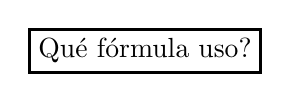
\begin{tikzpicture}
\node[draw, line width=0.04cm] at (8.4,2) {Qu\'e f\'ormula uso?};
\end{tikzpicture}
}

% ============================================================== 
%----------------------------------------------------------------
%----------------------------------------------------------------
\end{frame}


%________________________________________________________________(ult. col, 65)
% ========================== slide2 ============================= 
\begin{frame}
\frametitle{MRU}
% 
% -Paragraph1 
%----------------------------------------------------------------
%----------------------------------------------------------------
% -Idea1 
% ============================================================== 
 
{\huge                
\xmru
}                                             
 
% ============================================================== 
% -Idea2 
% ============================================================== 
 
Pero.. siempre debemos trabajar en el mismo sistema de unidades.
Es decir, si hay un kilometros/minutos,
debemos transformar los 
horas a minutos :)

%%%%%%%%%%%%%%%%%%%%%%%%%%%%%%%%%%%%%%%%%%%%%%%%%%%%%%%%%%%%%%%%
%%%%%%%%%%%%%%%%% Cajita de Texto sencilla %%%%%%%%%%%%%%%%%%%%%
\begin{center}
\fcolorbox{red}{red}{  % Simulated double frame with color
\parbox[c]{6cm}{
1 hora =  60 minutos \\
Entonces 90 horas son \\
90 $\times$ 60 minutos \\
90 horas =
5400 minutos.

}}
\end{center}
%%%%%%%%%%%%%%%%%%%%%%%%%%%%%%%%%%%%%%%%%%%%%%%%%%%%%%%%%%%%%%%%
%%%%%%%%%%%%%%%%%%%%%%%%%%%%%%%%%%%%%%%%%%%%%%%%%%%%%%%%%%%%%%%%
                           
% ============================================================== 
% -Idea3 
% ============================================================== 
 
Finalmente..                                                              
                                                               
                                                               
% ============================================================== 
%----------------------------------------------------------------
%----------------------------------------------------------------
\end{frame}


%________________________________________________________________(ult. col, 65)
% ========================== slide3 ============================= 
\begin{frame}
\frametitle{MRU}
% 
% -Paragraph1 
%----------------------------------------------------------------
%----------------------------------------------------------------
% -Idea1 
% ============================================================== 
{\large
\begin{equation}
x=
(3\frac{km}{\cancel{min}})
(5400\cancel{min})=
16200~km
\end{equation}}

                               
% ============================================================== 
% -Idea2 
% ============================================================== 
 
La distancia que recorre el objeto es
\fbox{16200 km}

                                                             
% ============================================================== 
% -Idea3 
% ============================================================== 
                                                               
                                                               
                                                               
% ============================================================== 
%----------------------------------------------------------------
%----------------------------------------------------------------
\end{frame}


%%%%%%%%%%%%%%%%%%%%%%%%%%%%%%%%%%%%%%%%%%%%%%%%%%%%%%
%%%%%%%%%%%%%%%  Tail  %%%%%%%%%%%%%%%%%%%%%%%%%%%%%%%
%%%%%%%%%%%%%%%%%%%%%%%%%%%%%%%%%%%%%%%%%%%%%%%%%%%%%%

\end{document}
%%
%% End of Beamer-ported file ==
%%
%% Modified 05-10-2008
